\section{Exploring the resolution speed}
\label{sec:question3}

\subsection*{Question 3.1}
\textit{What is the average resolution speed to an incident? Resolution speed is defined as the difference between the Event Clearance Date value (moment when the police closed the file of an incident) and the At Scene Time value (moment when the police arrived at the scene of the incident).}

The dataset does not define the average resolution time explicitly.
Thus, we need to add a new columns to the dataset with this information.
Tableau is able to compute new dimensions using the existing ones.
Since we compute a difference between $2$ timestamp, we use the function \texttt{datediff} to get a proper result.

The average resolution time of the entire dataset is about $2$ hours.

\begin{figure}[h]
	\centering
	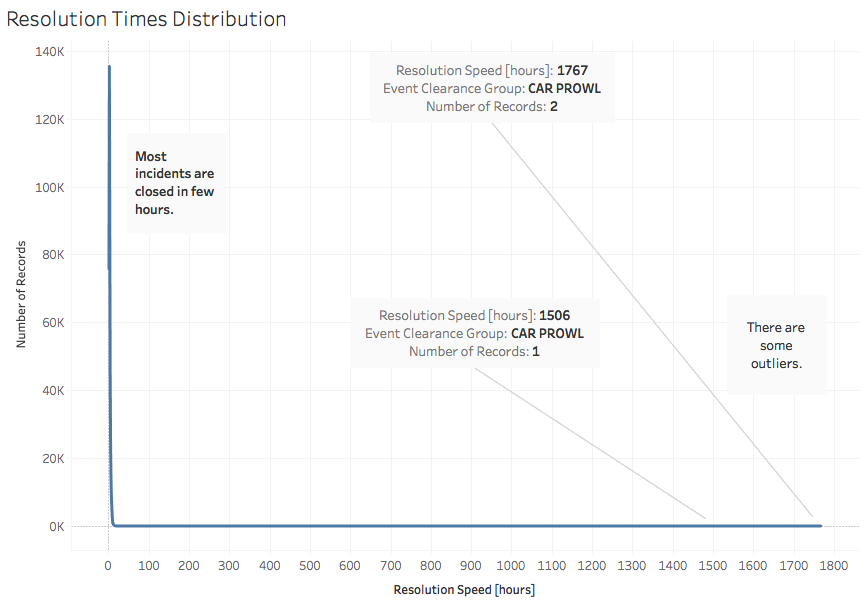
\includegraphics[width=0.9\columnwidth]{figures/3_1_resolution_speed_outliers}
	\caption{Distribution of the resolution times. The annotations on the plot show some outliers with very high resolution times. Most of the incidents are closed in few hours. This is a screenshot of sheet \textit{Resolution Times Distribution} in Tableau.}
	\label{fig:3_1_resolution_speed_outliers}
\end{figure}

\cref{fig:3_1_resolution_speed_outliers} shows the distribution of resolution times.
We can notice that:
\begin{itemize}
    \item Most incidents are closed in few hours.
    \item There are few outliers that have a resolution time of over $1500$ hours (approximately 2 months). All outliers share the same type: \textit{Car Prowl}.
\end{itemize}

The line chart gives already some interesting insides about incidents resolution times.
Due to the described outliers, it is difficult to read the left part of the chart, where most of the distribution mass is.

To solve the problem, we add an histogram of the resolution times.
Resolution time is a continuos measure, but we are not interested in the precise value for each incident, rather in the overall distribution.
To visualize the distribution, we discretize the resolution time in buckets of $1$ hour.
Since most of the density mass in the first $15$ buckets, we cut the histogram after the first $20$ ones.
Since we are loosing the outliers, we add a table that contains such information.

\cref{fig:3_1_resolution_speed} shows the final dashboard.
We can notice that:
\begin{itemize}
    \item The average resolution time is about $2$ hours.
    \item There are some outliers, but their number is really low in comparison to the amount of entries.
    \item Most incidents are closed in less than $10$ hours.
\end{itemize}

\begin{figure}[h]
	\centering
	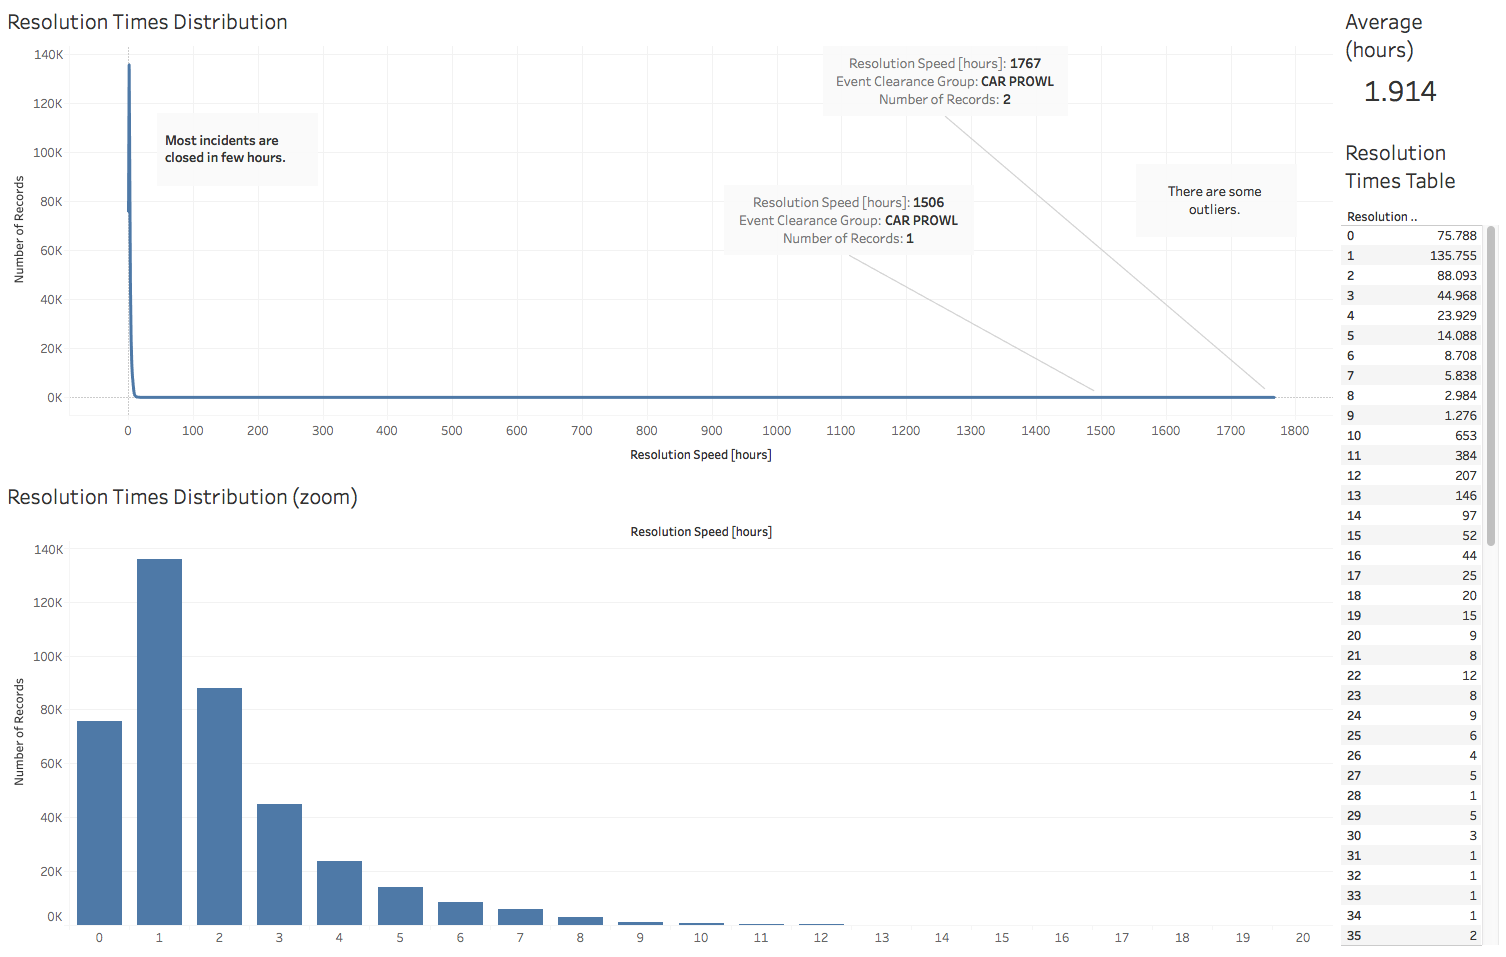
\includegraphics[width=\columnwidth]{figures/3_1_resolution_speed}
	\caption{Distribution of the resolution times. The dashboard is called \textit{Resolution Times} in Tableau.}
	\label{fig:3_1_resolution_speed}
\end{figure}


\subsection*{Question 3.2}
\textit{Are there certain types of incidents having a much lower resolution speed than others? If so, which are these?}

The visualization uses a bar chart.
Each type of is encoded in one bar and the height of the bar corresponds to the average resolution time for that type.
The types are ordered by average resolution time decreasing, so it is easy to spot the outliers.
Color is used to overload the encoding of the incident type.
The bar chart show the average line to make comparison and reasoning easier.
We prefer to use the x-axis for the type and the y-axis for the average resolution time since the visualization with swapped axises does not fit a single screen.

\cref{fig:3_2_resolution_speed_by_type} shows the visualization.
We can notice that:
\begin{itemize}
    \item \textit{Homicide} is the type with the highest average resolution time. This is not a surprise, since such an incident requires very accurate investigations.
    \item \textit{Public Gatherings} have the seconds highest average resolution time. This is probably due to the high number of people involved in the incident.
    \item \textit{Vice Calls} have the fastest resolution time, on average only about $30$ minutes.
    \item \textit{False Alarms} are also resolved quite fast, less than $1$ hour on average.
    \item All other types have resolution times between $1$ and $3$ hours on average.
    \item The distribution is skewed to towards types with higher resolution times.
\end{itemize}

\begin{figure}[h]
	\centering
	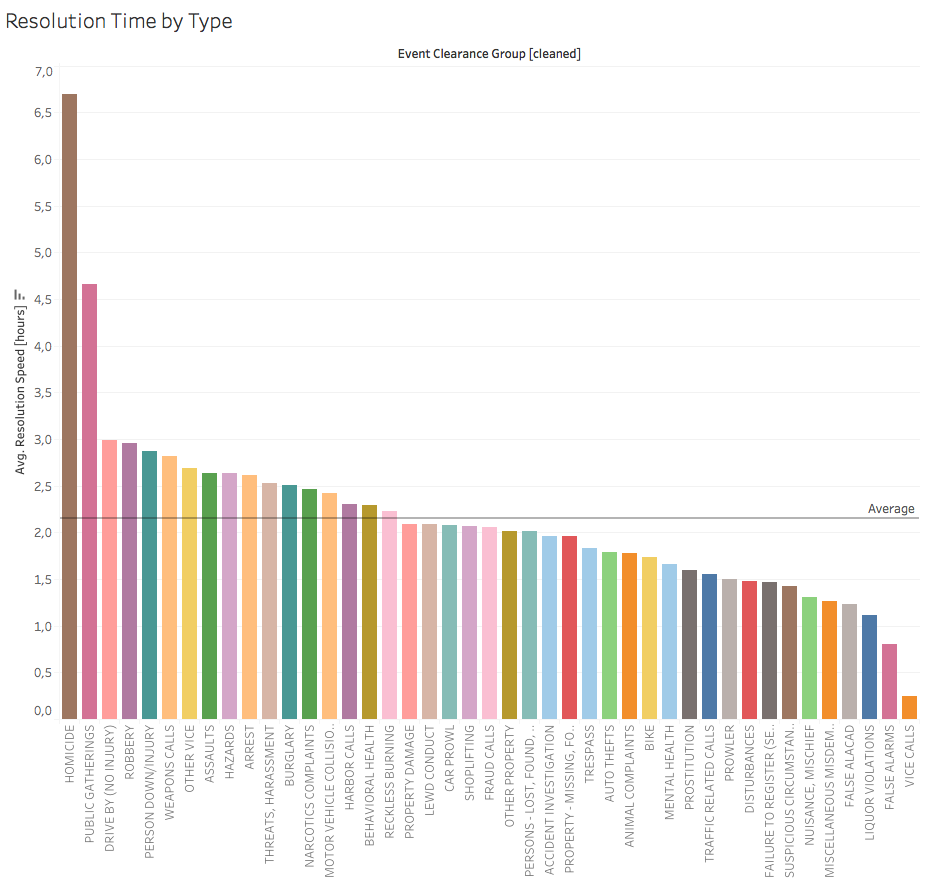
\includegraphics[width=\columnwidth]{figures/3_2_resolution_speed_by_type}
	\caption{Incidents' resolution time by type. The sheet is called \textit{Resolution Time by Type} in Tableau.}
	\label{fig:3_2_resolution_speed_by_type}
\end{figure}


\subsection*{Question 3.3}
\textit{Does the resolution speed depend on the time period (e.g., year, season of the year)?}

The visualization uses a scatterplot to visualize the resolution speed of incidents over time.
The x-axis encode the time at scene, the y-axis the resolution speed in hours.
We use color to overload the encoding of the resolution speed.
In particular, we use a continuos heat colormap.
We show the average line in order to be able to compare time ranges with the average behaviour.

\begin{figure}[h]
	\centering
	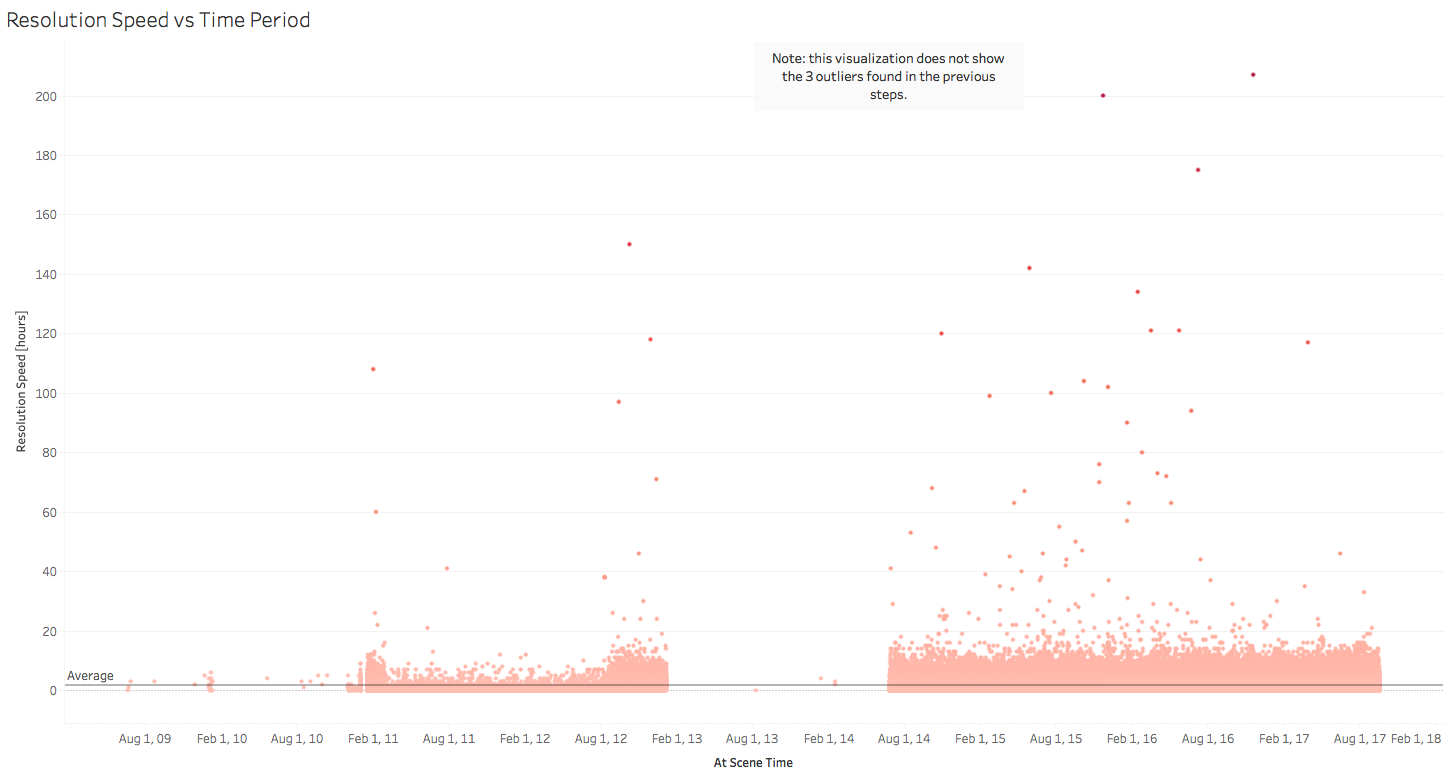
\includegraphics[width=\columnwidth]{figures/3_3_resolution_speed_vs_time}
	\caption{Incidents' resolution speed over time. Please note that the $3$ outliers cited in the text are excluded from this visualization. The sheet is called \textit{Resolution Speed vs Time} in Tableau.}
	\label{fig:3_3_resolution_speed_vs_time}
\end{figure}

The visualization is difficult to read due to the presence of the $3$ outliers described in Question 3.1.
Since we have discussed them already, we remove them from this visualization.
The result is shown is \cref{fig:3_3_resolution_speed_vs_time}:
\begin{itemize}
    \item There are $4$ slots of times that appears differently. The $1^{st}$ (02/2009 - 01/2010) and $3^{rd}$ (02/2013 - 07/2014) slots have almost no data. There is not much we can say about those periods.
    \item The $2^{nd}$ slot (02/2011 - 01/2013) has a period where incidents are resolved faster, in particular from 03/2011 to 08/2012; in this period most incidents are closed in less than $2$ hours.
    \item The $4^{th}$ slot (08/2014 - 09/2017) seems to have a uniform distribution for the resolution speeds, with an average higher than the $2^{nd}$ slot.
\end{itemize}

Overall, the resolution speed seems to be not correlated to the particular period of the year (i.e. month or season).
To confirm this hypothesis, we create $2$ new bar charts that show respectively the average resolution speed by season and by month.
We use color to overload the encoding of the values showed by the bars to make the plots easier to read.
We also create $2$ bar charts to show the number of incidents by season and month, to make sure that the number of incidents does not vary significantly over the year (since this would probably affect the average resolution speed).
From \cref{fig:3_3_resolution_speed_by_season_and_month} we can confirm that there is no significant correlation between the period of the year and the incidents' resolution speed.
Also, we can notice that there is a higher number of incidents during the summer period (July, August and September);
however, this does not influence the average resolution speed.
The scatterplot and the bar charts are grouped in the \textit{Resolution Speed} dashboard.

\begin{figure}[h!]
    \begin{subfigure}{0.45\textwidth}
        \centering
        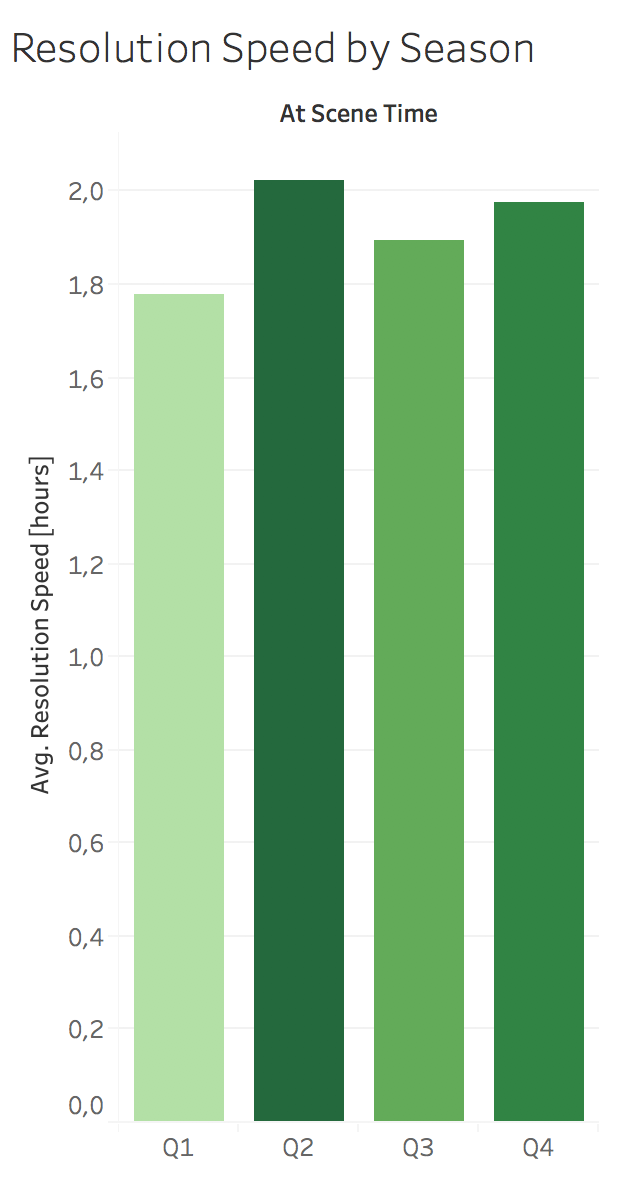
\includegraphics[width=0.532\linewidth]{figures/3_3_resolution_speed_by_season} 
        \caption{Resolution speed by season.}
        \label{fig:3_3_resolution_speed_by_season}
        \vspace*{5mm}
    \end{subfigure}
    \begin{subfigure}{0.55\textwidth}
        \centering
        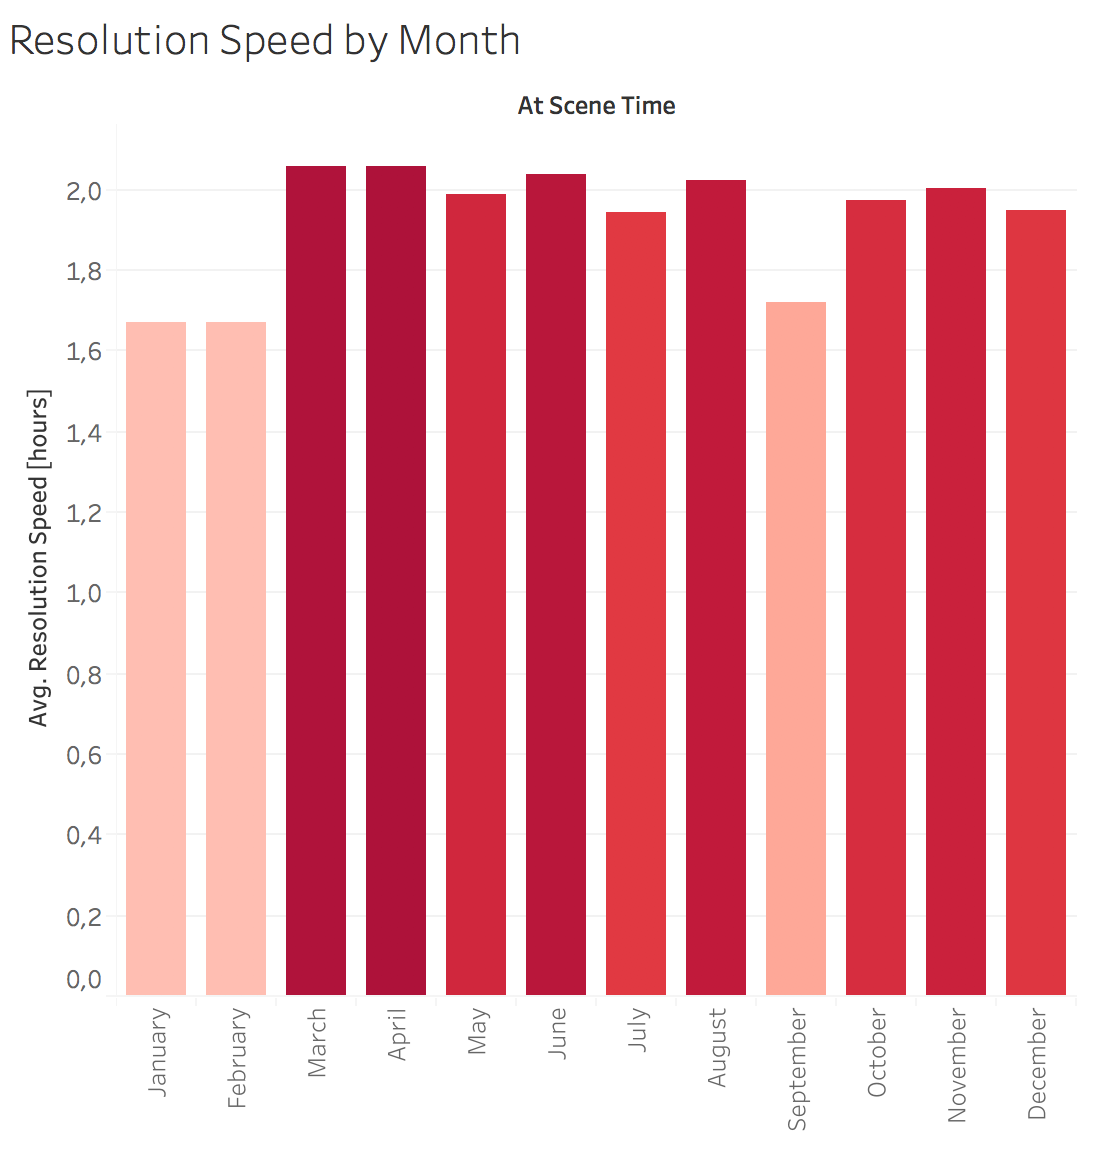
\includegraphics[width=0.8\linewidth]{figures/3_3_resolution_speed_by_month}
        \caption{Resolution speed by month.}
        \label{fig:3_3_resolution_speed_by_month}
        \vspace*{5mm}        
    \end{subfigure}
    \begin{subfigure}{0.45\textwidth}
        \centering
        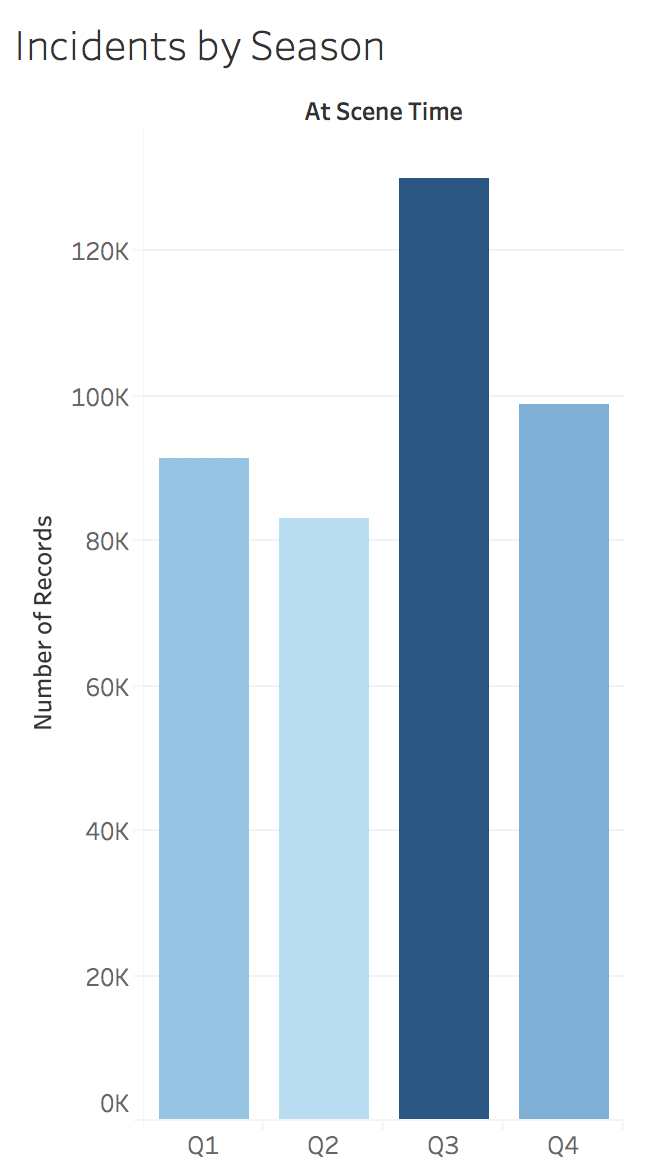
\includegraphics[width=0.562\linewidth]{figures/3_3_incidents_by_season} 
        \caption{Number of incidents by season.}
        \label{fig:3_3_resolution_speed_by_season}
        \vspace*{3mm}        
    \end{subfigure}
    \begin{subfigure}{0.55\textwidth}
        \centering
        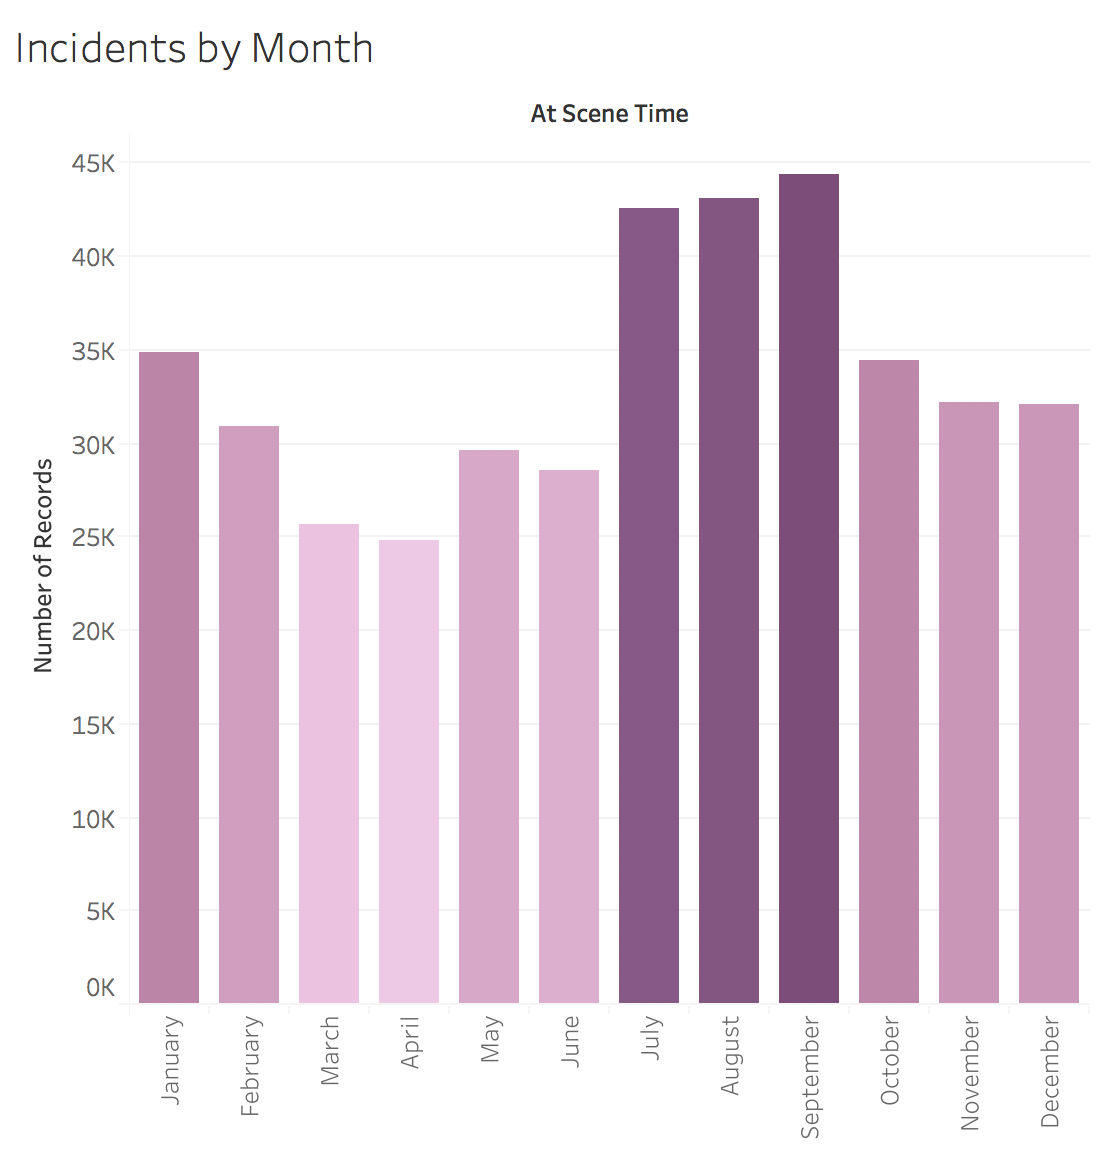
\includegraphics[width=0.8\linewidth]{figures/3_3_incidents_by_month}
        \caption{Number of incidents by month.}
        \label{fig:3_3_resolution_speed_by_month}
        \vspace*{3mm}        
    \end{subfigure}
    \caption{Overview of the resolution speed and number of incidents by season and month. The bar chart are grouped in the \textit{Resolution Speed} dashboard in Tableau.}
    \label{fig:3_3_resolution_speed_by_season_and_month}
\end{figure}
